\newpage
\section{Realisering}
\label{realiseringOgTest}

\subsection[short]{Bestemme verdier}
\label{bestemmeVerdier}

For å bestemme verdiene til komponentene i kretsen så må det først bestemmes hvilke krav som stilles til kretsen. Det er ønskelig med så høy ingangsmotstand og så lav utgangsmotstand som mulig og at kretsen skal kunne levere mye strøm. %OPA454 er en moderne høy strøms operasjonsforsterker som kan levere 50mA. 
Det er derfor ønskelig at kretsen skal kunne levere minst 50mA.

Vi starter med å definere arbeidspunktet og $I_E$. Arbeidspunktet settes til midten av spenningsforsyningen, pluss . $I_E$ settes til 50m, og arbeidspunktet settes ved å bruke formel \ref{eq:arbeidspunkt}. 

\begin{equation}
\label{eq:arbeidspunkt}
\begin{split}
V_B &= \frac{V_{CC} - V_{BE}}{2} + V_{BE}\\
V_B &= \frac{7V - 1,4V}{2} + 1,4V = 4.2V
\end{split}
\end{equation}

\begin{equation}
\label{eq:IE}
\begin{split}
I_{E1} &= I_{C1} + I_{B}\\
I_{E1} &= I_{B}(\beta + 1)\\
I_{E} &= I_{C2} + I_{E1}\\
I_{E} &= I_{B}(\beta + 1)^2 \\
\end{split}
\end{equation}

\begin{equation}
\label{eq:IB}
\begin{split}
I_{B} &= \frac{I_{E}}{(\beta + 1)^2} \\
I_{B} &= \frac{50mA}{(330 + 1)^2} = 0.45\mu A
\end{split}
\end{equation}

\begin{equation}
\label{eq:R1}
\begin{split}
R_{1} &= \frac{V_{CC} - V_{B}}{I_{B}}\\
R_{1} &= \frac{7V - 4.2V}{1000*0.45\mu A} = 6.2k\Omega
\end{split}
\end{equation}

\begin{equation}
\label{eq:R2}
\begin{split}
V_{R2} &= \frac{V_{CC} R_2}{R_1 + R_2}\\
R_2 &= \frac{V_{R2} R_1}{V_{CC}-V_{R2}}\\
R_2 &= \frac{4.2V 6.2k\Omega}{7V-4.2V} = 9.3k\Omega
\end{split}
\end{equation}

\begin{equation}
\label{eq:RE}
\begin{split}
R_{E} &= \frac{V_{B}}{I_{E}}?\\ 
\end{split}
\end{equation}



\vspace{1cm}
\begin{table}[!h]
\centering % Denne kommandoen sentrerer tabellen i kolonnen. 
\caption{Beregna verdier.}
\label{tab:vars}	% Merkelappen vi vil referere til.
\begin{tabular}{lll} % Her angir det andre argumentet at vi vil ha to senterjusterte kolonner (l = left, c = center, r = right).
\toprule % Horisontal linje som markerer toppen av tabellen
\textbf{Variabel/komponent} & \textbf{Verdi} & \textbf{Kommentar} \\
\midrule
$V_{\text{CC}}$ & $6\text{V}$ & \\
$V_\text{T}$ & $0.7\text{V}$ & \\
$R_{\text{B}2}$ & $470\text{k}\Omega$ & inngangsimpedansen må være høy i en buffer \\
$I_\text{E}$ & $10\text{mA}$ & \\
$V_\text{B}$ & $4.2\text{V}$ & \\
$R_{\text{B}1}$ & $690\text{k}\Omega$ & \\
$R_\text{E}$ & $330\Omega$ & utgangsimpedansen er lav i en buffer \\
$C_1$ & $1\mu\text{F}$ & \\
$C_2$ & $1\mu\text{F}$ & \\
\bottomrule 
\end{tabular}
\end{table}
\vspace{1cm}

\subsection{Oppkobling og test}
Kretsen ble deretter koblet opp i henhold til skjematikken i figur \ref{fig:Darlington_buffer} med verdiene fra tabellen i figur \ref{tab:vars}. For å få $V_{CC}$ på 7V så ble spenningsforsyningen på Analog Discovery satt til +5V og gjord ble satt til -2V.

\begin{figure}[H]
\centering
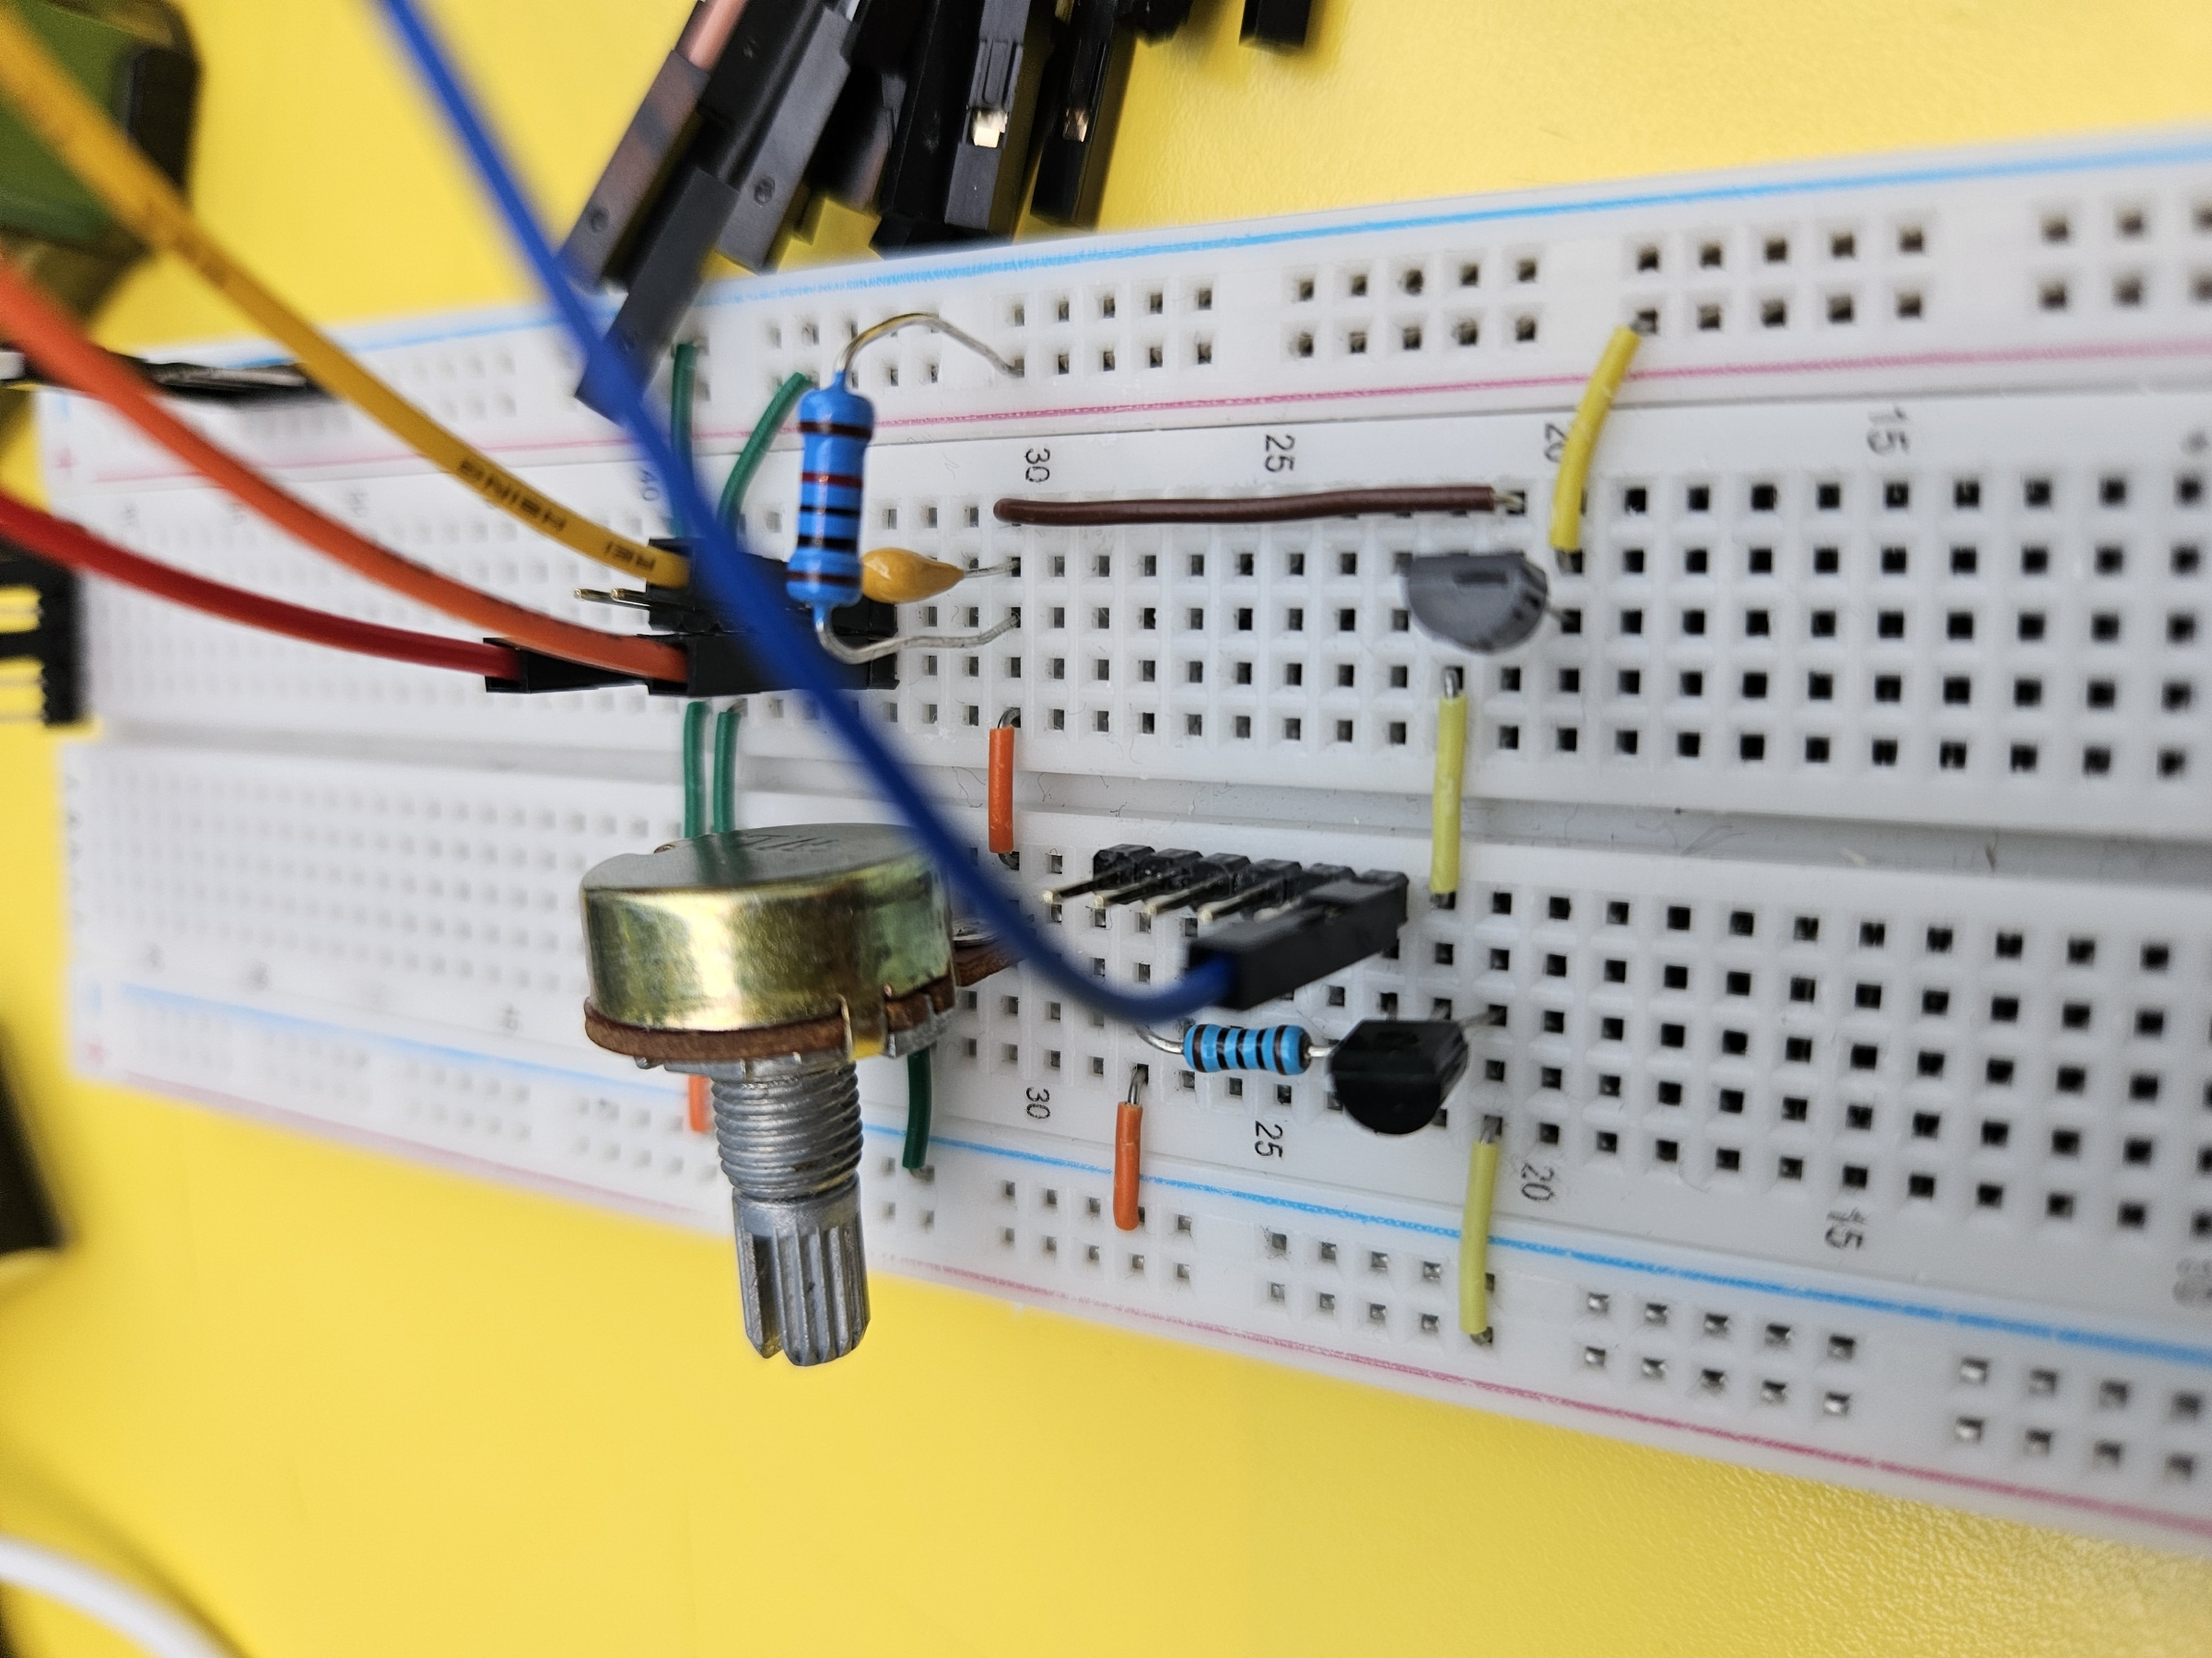
\includegraphics[scale=0.1]{bilder/Oppkobling.jpg}
\caption{Reailsert og oppkoblet krets}
\label{fig:Oppkobling}
\end{figure}


\subsubsection{Test under ideelle forhold}

Kretsen ble først testet uten last og kildemotstand for å se om den fungerte som forventet. Det ble da målt en forsterkning på EDIT og en faseforskyvning på EDIT grader. Dette er innenfor det som er forventet og kan ses i figur \ref{fig:Bodeplot+Pase_First} Hvor V er ingagnsignalet og V2 er utgangssignalet.

\begin{figure}[H]
\centering
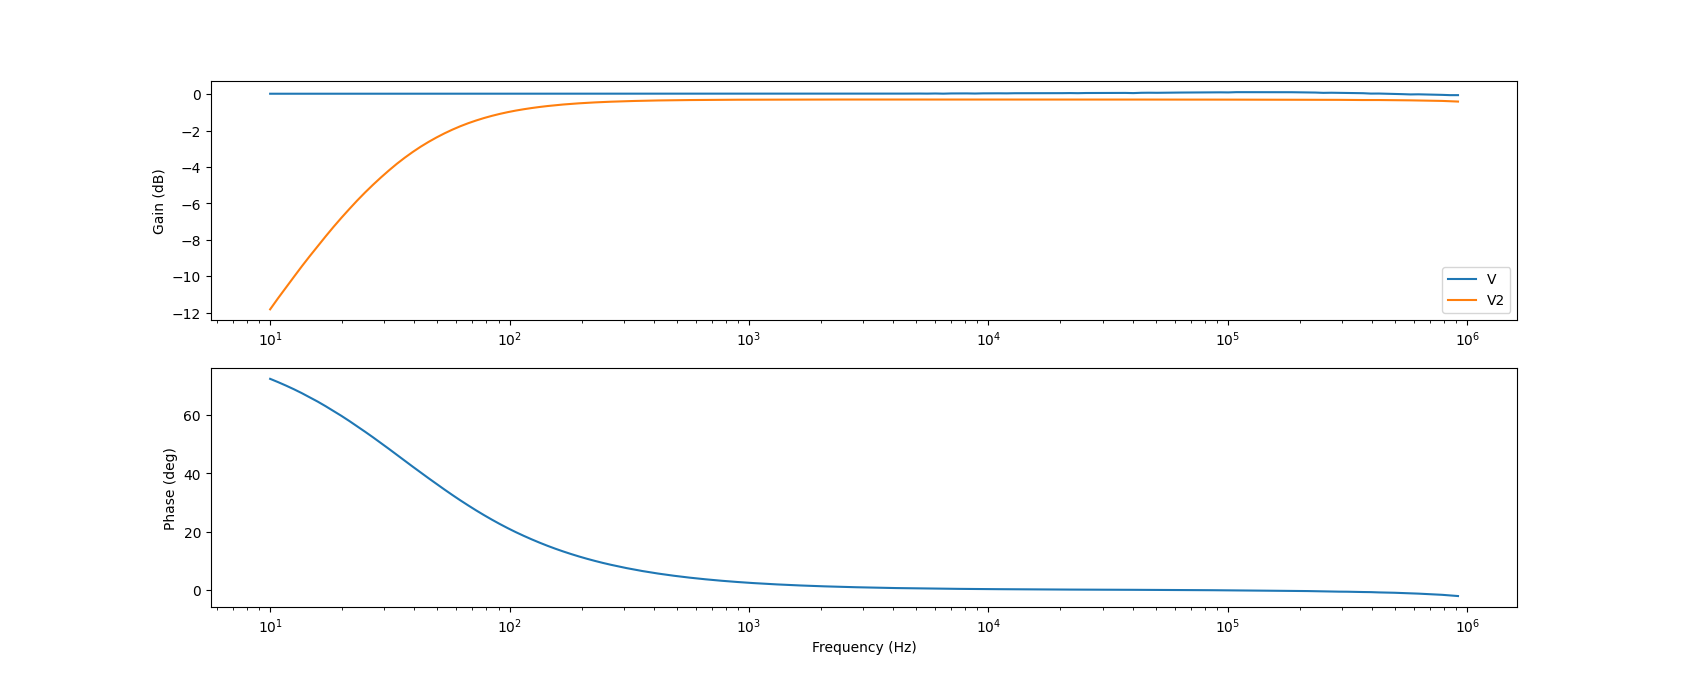
\includegraphics[scale=0.4]{bilder/Bodeplot+Pase_First.png}
\caption{Bodeplot under ideelle forhold}
\label{fig:Bodeplot+Pase_First}
\end{figure}


\subsubsection{Test med last}

Så ble latstmotstand og kildemotstand koblet til kretsen. Kildemotstanden ble satt til 1.5k$\Omega$ og lastmotstanden ble satt til 170$\Omega$. Som vist i figur \ref{fig:Bodeplot+Pase_Second} så økte forvregningen av signalet. For å forbedre dette så ble det byttet til større kondensatorer, fra $1\mu$F til $16\mu$F og inngangsmotstanden ble økt ved å gange $R_1$ og $R_2$ med 100. Deretter ble det målt en forsterkning på EDIT og en faseforskyvning på EDIT grader. Dette kan ses i figur \ref{fig:Third}.

\begin{figure}[H]
\centering
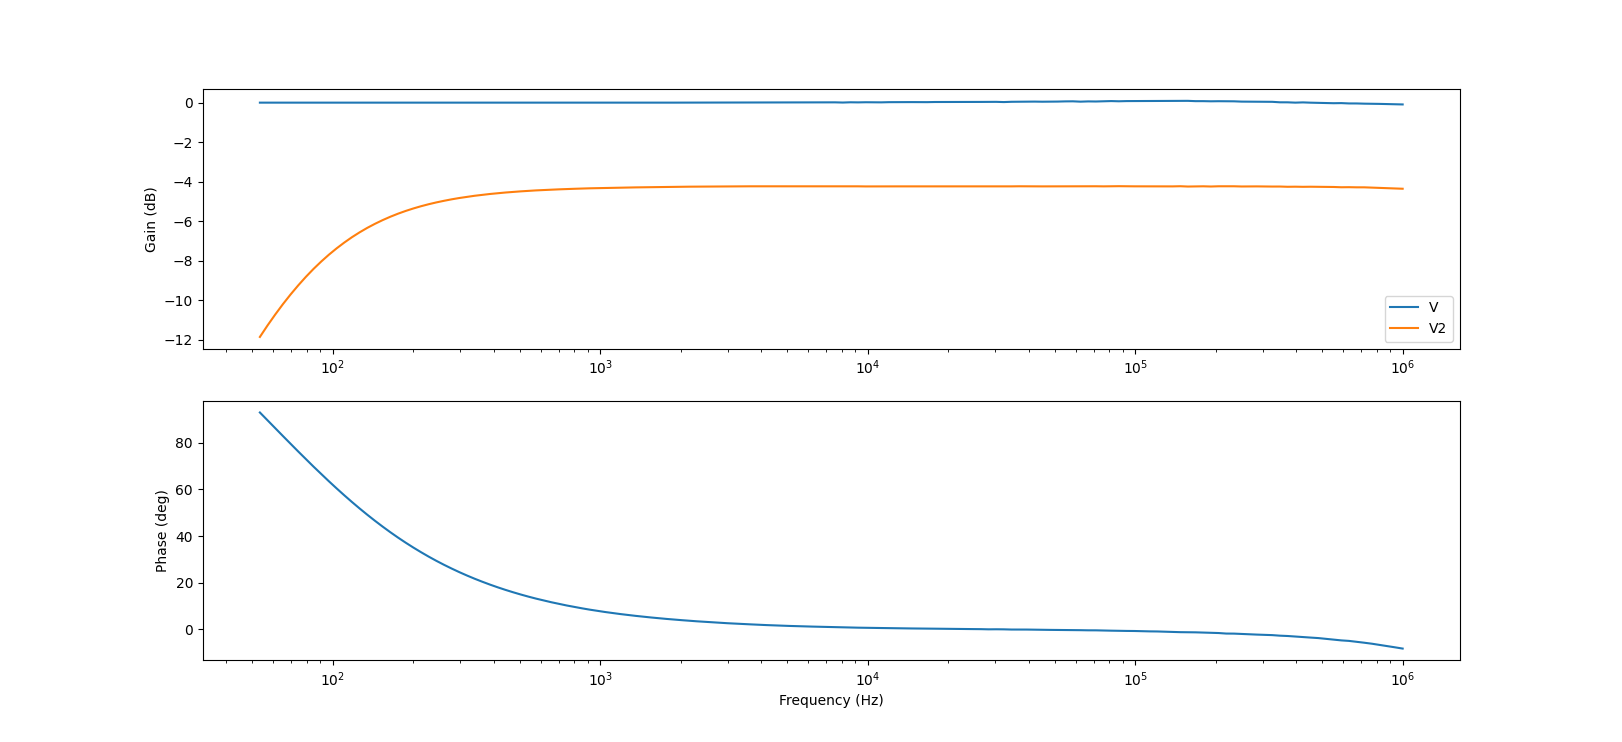
\includegraphics[scale=0.4]{bilder/Bodeplot+Pase_Second.png}
\caption{Bodeplot med last}
\label{fig:Bodeplot+Pase_Second}
\end{figure}

\begin{figure}[H]
\centering
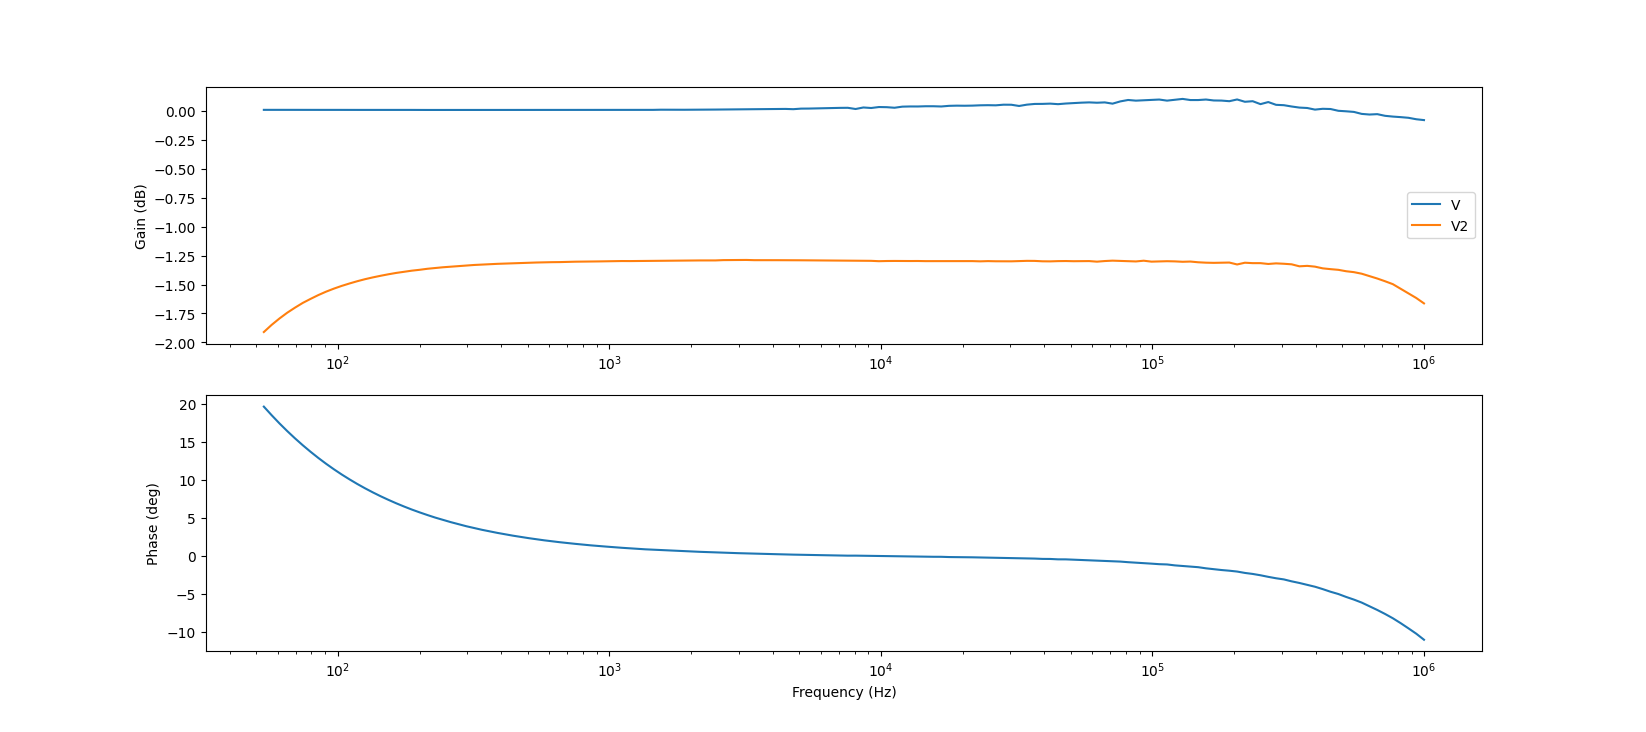
\includegraphics[scale=0.4]{bilder/Bodeplot+Pase_Third.png}
\caption{Last}
\label{fig:Third}
\end{figure}

Ved å utvide network målingen til å måle fra 1Hz til 5MHz så kan vi finne knekkfrekvensen til kretsen. Nedre knekkfrekvens er 24Hz og øvre knekkfrekvens er 2.7MHz. Dette kan ses i figur \ref{fig:Last+Pase}.

\begin{figure}[H]
\centering
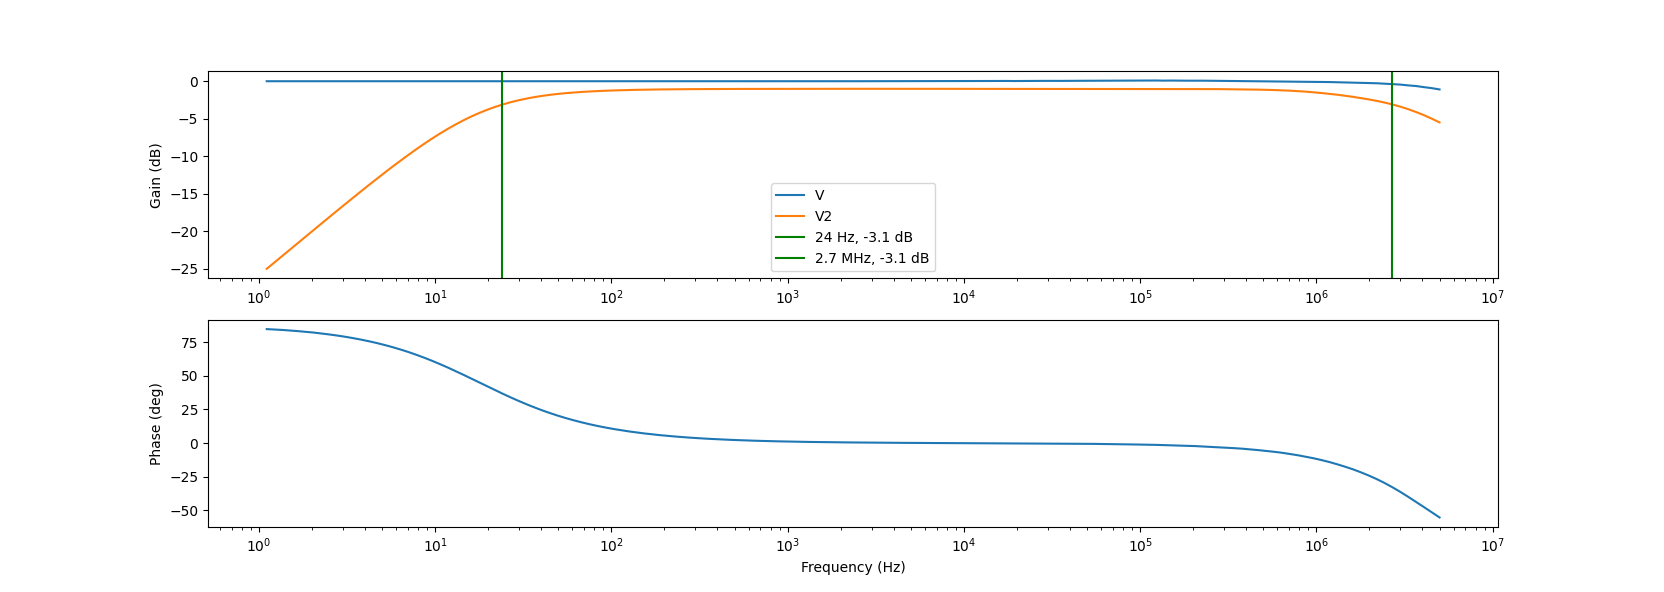
\includegraphics[scale=0.4]{bilder/Bodeplot+Pase_Last.png}
\caption{Last med fase}
\label{fig:Last+Pase}
\end{figure}



%Two png files next to each other

\begin{figure}[H]
    \centering
    \begin{minipage}[c]{0.49\textwidth}
        \centering
        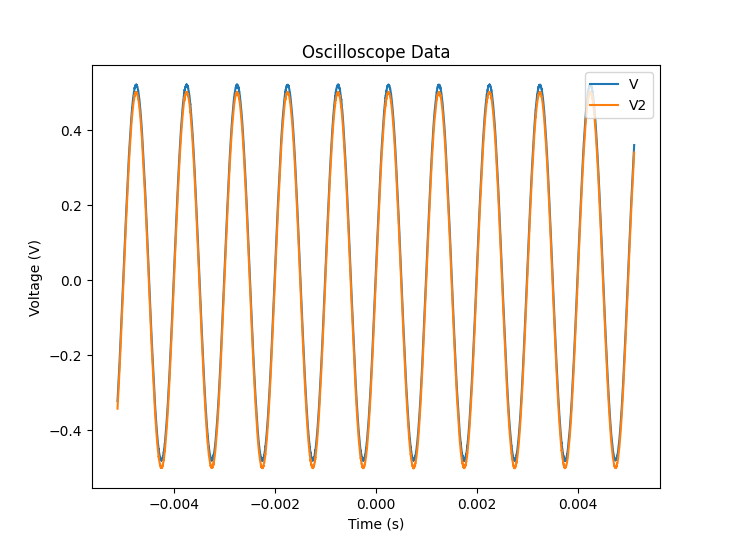
\includegraphics[width=1\textwidth]{Bilder/Scope_Nice.png} 
        \caption{1kHz ved 500mV og klipping ved 1V}
        \label{fig:Scope_Nice}
    \end{minipage}
    \hfill
    \begin{minipage}[c]{0.49\textwidth}
        \centering
        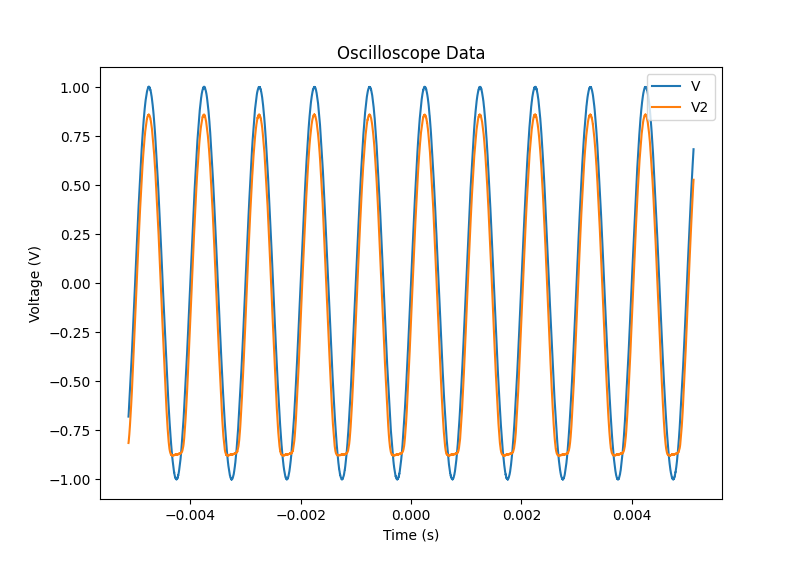
\includegraphics[width=1\textwidth]{Bilder/Scope_Unice.png} 
        \label{fig:Scope_Unice}
    \end{minipage}
\end{figure}
